\documentclass[journal,a4paper]{IEEEtran}

% to typeset URLs, URIs, and DOIs
\usepackage[english]{babel}
\usepackage{url}
\usepackage{multicol}
\usepackage{multirow}
\usepackage{url,hyperref,graphicx,float,times}
\usepackage{textcomp}
\usepackage{cite}
\usepackage[caption=false,font=footnotesize]{subfig}
\usepackage{amsmath}
\graphicspath{ {./images/} }


\begin{document}
%
\title{Decentralized Data Marketplace to Enable Trusted Machine Economy}
%
\author{
%%% Fill in name here
\IEEEauthorblockN{Zan-Jun Wang\IEEEauthorrefmark{3}, Ching-Hua Lin\IEEEauthorrefmark{2}, Yang-Hao Yuan\IEEEauthorrefmark{4}, Ching-Chun (Jim) Huang\IEEEauthorrefmark{1}}\\

%%% Fill in school here
\IEEEauthorblockA{\IEEEauthorrefmark{1}\IEEEauthorrefmark{2}Department of Computer Science and Information Engineering, National Cheng Kung University} \\
\IEEEauthorblockA{\IEEEauthorrefmark{3}Department of Computer Science and Information Engineering, National Taiwan University} \\
\IEEEauthorblockA{\IEEEauthorrefmark{4}BiiLabs, Co., Ltd.} \\

%%% Fill in address here
\IEEEauthorblockA{\IEEEauthorrefmark{1}\IEEEauthorrefmark{2}No.1, University Road, \IEEEauthorrefmark{3}No.1, Sec. 4, Roosevelt Road} \\

%%% Fill in city and country here
\IEEEauthorblockA{\IEEEauthorrefmark{1}\IEEEauthorrefmark{2}Tainan City, Taiwan (R.O.C.), \IEEEauthorrefmark{3}Taipei City, Taiwan (R.O.C.)} \\

%%% Fill in email here
\IEEEauthorblockA{\IEEEauthorrefmark{1}jserv@ccns.ncku.edu.tw, \IEEEauthorrefmark{2}jkrvivian@gmail.com, \IEEEauthorrefmark{3}twzjwang@gmail.com, \IEEEauthorrefmark{4}yanghau@biilabs.io}
}


%


\maketitle              
% 50-80 words
\begin{abstract}
abstract here
\end{abstract}

% 3 - 4 keywords
\begin{IEEEkeywords}
streaming data, crowd sensing, data marketplace, decentralization
\end{IEEEkeywords}

\section{Introduction}

\section{Related Work}
The economic value of huge amount of data emerges, several researchers have started to explore the design of data marketplace. The Third Party Auditors (TPAs)-based frameworks is far from being satisfactory due to the unstandardize data format and dynamic nature of IoT data. Therefore a decentralized data integrity validation and trading process has been proposed recent years, and blockchain is considered a solution.

Data Integrity as a Service (DIaaS) is a blockchain based framework for data integrity proposed by Liu et al.\cite{DIaas} which is a Cloud Server Service (CSS) allows both data provider and consumer to validate data integrity by comparing hashes on Ethereum smart contract and Cloud Server. Moreover, Ethereum smart contract can also realize the purchase agreement, including authoriziation and the penalization. However, the architecture of DIaaS needs highly trust on CSS, if CSS is malicious or crashed, that will cause losses to both providers and consumers. Also, the performance analysis shows that IoT devices have low efficiency interacting with Etheruem due to the time-consuming Proof-of-Work(PoW) process.

By solving the inefficiency of the Blockchain, \textbf{IOTA}\cite{IOTAwhitepaper} is a cryptocurrency for the IoT industry based on a revolutionary distributed ledger technology, the \textbf{Tangle}, which enables zero-transaction. On top of that, \textbf{Masked Authenticated Messaging(MAM)}\cite{MAM}, a second layer data communication protocol which allows to emit and access an encrypted data stream over the Tangle where privacy and integrity meet. 

On the basis of the Tangle and MAM, IOTA foundation proposed a decentralized Data Marketplace\cite{IOTADataMarket} which is suitable for IoT streaming data that not only allows data providers to put data on Tangle without any trusted cloud services, but also allow providers and consumers to trade on Tangle and protect privacy and assure data integrity from source with MAM. Nevertheless, the platform design is centralized, new devices require manual approval from IOTA team to be visible in the marketplace. Also, interacting with Tangle is still the bottleneck for low-level devices especially in an unstable network or electricity environment.

A different framework design proposed by Gupta, S.Kanhere and Jurdak\cite{3tierDataMarket} could reduce the burden of low-level devices as mentioned. The infrastructure is a 3-tier decentralized data marketplace architectural design with Ethereum smart contract which consists of provider, consumer and broker. Where broker is a highly resourced and trustless device that will facilitate the trading of data between the consumer and providers. However, the data integrity and authentication of each participant are still future work.  

The authors want to ensure the sustainability of decentralized data marketplace. The utility structure of IoT econimic system and game theory models are presented in the work of Dusit Niyato et al.\cite{UtilityStruct}. Game theory provides a mathematical solution to proof the existence of Nash Equilibrium in IoT economy. data marketplace organizers can apply numerical analysis on game theory, which would help them to find out their optimal pofit.

The previous work proposed different solution to specific issues of data marketplace. In this paper, we proposed an  overall design of decentralized data markeplace that takes care of data integrity and trading procedure such as buyout and subsciption on distributed ledger.

\section{System Architecture}
Our proposed data marketplace framework is a 3-tier decentralized and trustless architecture with a registrar who is responsible for marketplace registration in order to put participants' information on distributed ledgers for validation, brokers who interact between data providers and consumers, including data uploading, product metadata generation and trading process, data providers who upload data, and data consumers who search for interested products and issue a new trade.

\subsection{Participants}
There are four major roles in the decentralized data marketplace (Figure \ref{fig:system_design}).

\subsubsection{Registrar}
Registrar is responsible for creating a Registration Contract, which maintains a lookup table of participants, and adding new data providers, consumers and brokers to the decentralized data marketplace.

\subsubsection{Data Provider}
Data providers, who generate and preserve IoT data, are willing to sell sensing data to consumers. They decide the subscription period, subscription price, data type, sampling frequency. Afterward, they can launch the product on the decentralized data marketplace. Next, they collect raw data with their sensors and send to the broker who assists in uploading data to the network. An MAM channel\cite{MAM} is used to store encrypted data stream.

\subsubsection{Consumer}
Consumers aspire to obtain IoT data to promote the value of their service. However, it is a big challenge for most consumers to collect the desired data by themselves. So they look forward to purchasing the IoT data from data providers.

\subsubsection{Broker}
Brokers represent data providers and consumers to do computing tasks in the DLT (Distributed Ledger Technology) since brokers are expected to have high computing power. Once a data provider wants to launch a new product, the data provider requests a broker to create a new MAM channel, a new Product Contract, which specifies details about products, and upload this product to the IPFS (InterPlanetary File System)\cite{IPFS}. Also the broker certifies the session key which is used for symmetric encryption for streaming data encryption and decryption. Then the broker provides the matching service for data provider’s products and consumer’s queries. After that, the broker is requested to deal with the trading process and upload the provider’s data streams to the MAM channel.

\begin{figure}[h]
	\centering
	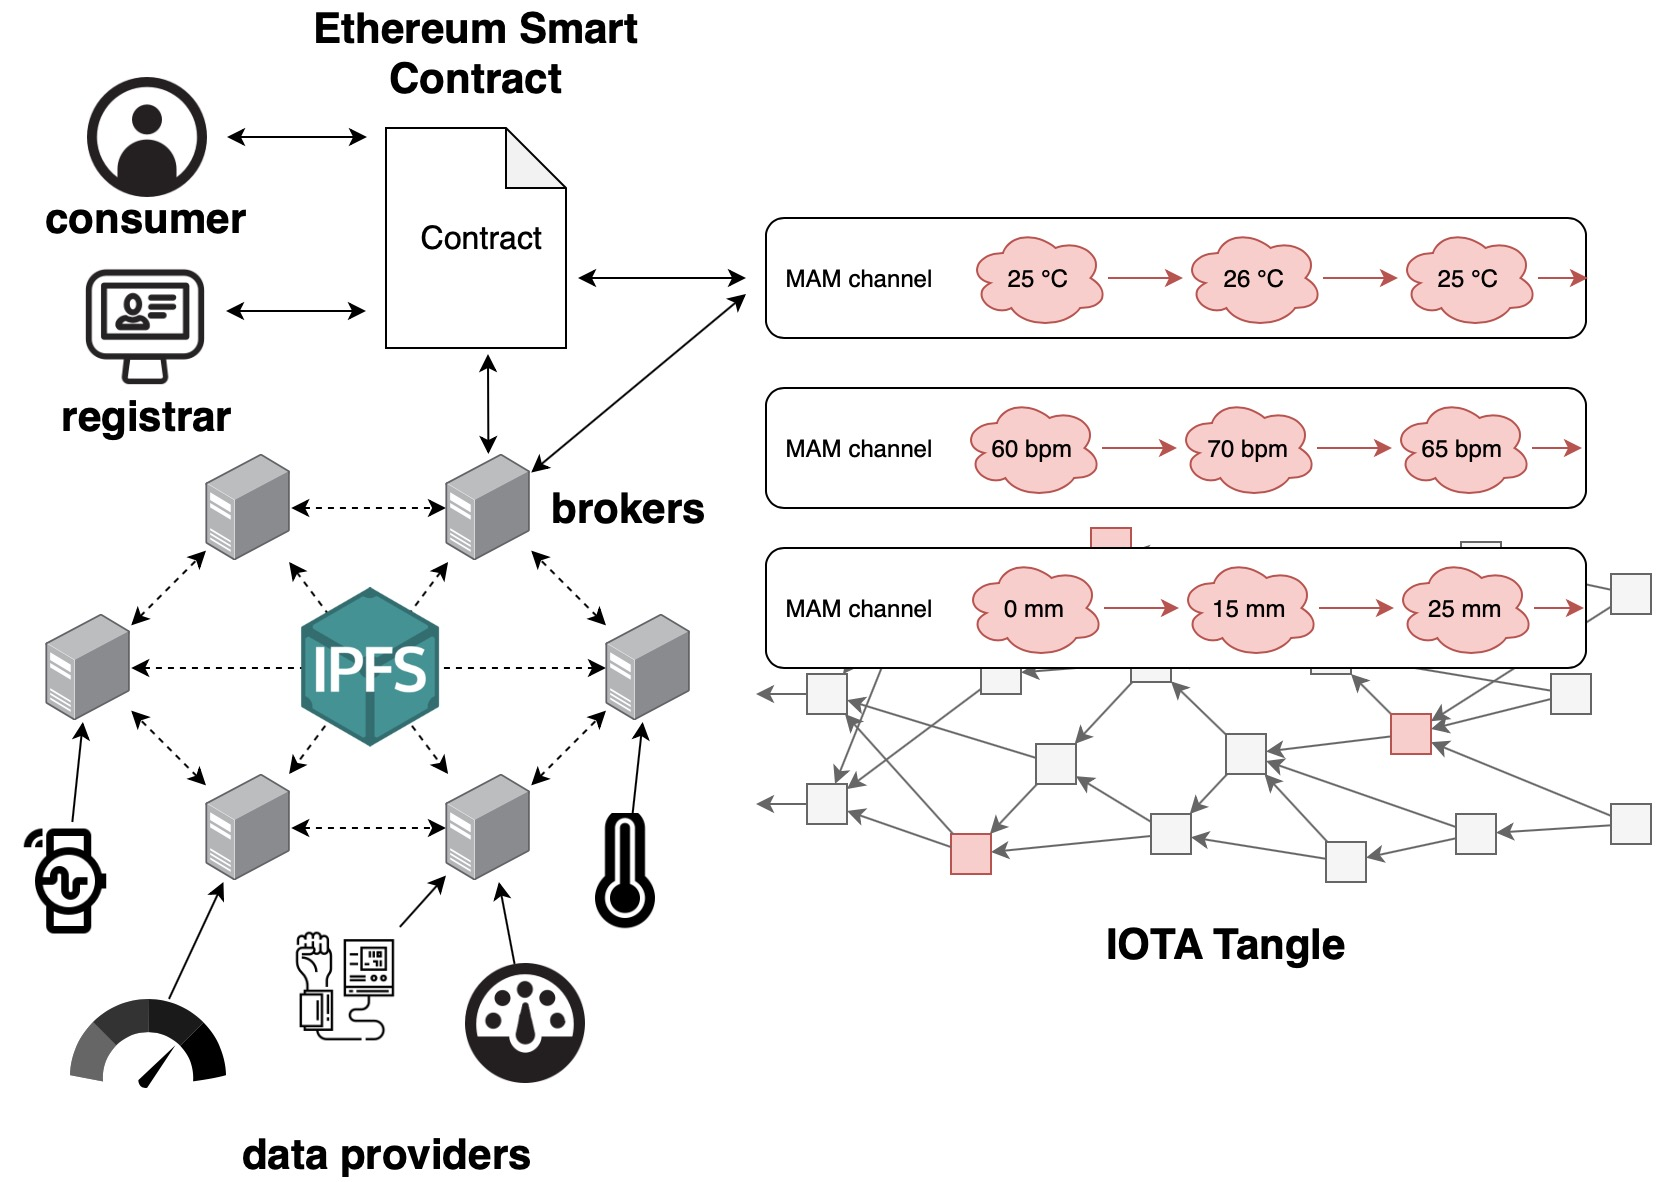
\includegraphics[width=0.4\textwidth]{system_design}
	\caption{System Design.}
	\label{fig:system_design}
\end{figure}

\subsection{Component}
\subsubsection{IOTA}
IOTA\cite{IOTAwhitepaper} is a cryptocurrency which the ledger does not consist of transactions grouped into blocks and stored in sequential chains, but a directed acyclic graph(DAG) of individual transactions, \textbf{Tangle}. To issue a transaction in the network, one needs to perform a small amount of Proof-of-Work (PoW) that verifies two previous transactions. Since every actor in Tangle has the same role, there is no need to offer transaction fees. Therefore, it is possible to make \textbf{micropayments} which the importance will increase in the rapidly developing IoT industry, and \textbf{zero-transactions} that one could store information securely within Tangle transactions. Moreover, this structure also enables high scalability of transactions that could resolve the drawbacks of blockchain and the concern of rapid growth of IoT devices.

\subsubsection{Ethereum Smart Contract}
Smart contract\cite{smartContract} is a protocol for formulating agreement on blockchain that provides verification and execution of the contract. The code in the smart contract could interact with other contracts, make decisions, store data and transfer cryptocurrency. All conditions and states established in the contract are transparent and with enforcement. The appearance of smart contracts makes trading more flexible, and achieves more complex trading patterns in reality.

\subsubsection{IPFS}
Inter-Planetary File system(IPFS)\cite{IPFS} is a peer-to-peer network for storing and accessing files, websites, applications, and data in a distributed file system which is not maintained with certain nodes or entities but all IPFS users. In our proposed architecture, brokers are responsible to upload the metadata of products, including title, data provider information and data preview to IPFS in order to provide users with search capabilities to meet the consumers' need.

\subsubsection{Masked Authenticated Messaging}
MAM\cite{MAM} is one of the best features of IOTA, it is a second layer data communication protocol enables to emit and access an encrypted data stream over Tangle network. The consensus algorithm of IOTA ensures data integrity. These properties allow MAM to meet the requirements of both data integrity and privacy.

IOTA only allows one message per transaction and couldn't publish continuous related messages because it is easy for an attacker to issue spam transactions if the same address is used. However, MAM publishes each message to a different addresses, and each can be derived from the previous one, this mechanism protects the channel from spamming and allows us to have access to all information with channel root only. Furthermore, MAM can be used in 3 ways to control visibility and access which are public, restricted and private. In our system, restricted MAM channel is used to achieve data authoriazation between providers and consumers.

\subsubsection{TangleID}
TangleID\cite{TangleID} is a self-soverign identity system based on IOTA, the goal is to establish a solution that do not require any third-party authority to verify an identity and its digital footprint. In TangleID, the digital footprint is converted into digital assets with the principle of Decentralized Identifiers (DIDs)\cite{DID} defined by W3C, and by putting DID documents on MAM makes TangleID a GDPR-Complianced system. Each identity has a public/private key pair recorded on MAM, it is used in digital signature for identity authentication. With every participant in data marketplace registers on TangleID, one can easily verify data provider's identity and data integrity with the public key on the DID document, and that we can ensure the reliability of data sources.


\subsubsection{Blind Signature}
Blind signature\cite{blindSig} is a form of digital signature where the message is blinded before it is signed, and the resulting blind signature can be verified publicly against the original. To perform such a signature, the message is first "blinded" by a random "blinding factor", then passed to a signer to sign. The resulting message, along with the blinding factor, can be later verified with the signer's public key. In our system design, brokers would perform blind signature during the process of adding new products for data providers, in order to upload the secret key of MAM channel to smart contract without knowing it. Furthermore, only one blind-signatured secret key is valid for trading and it is not allowed to be updated. By putting the secret key on smart contract prevents malicious providers trades invalid secret keys to consumers privately. 

\section{Trading Model}
In the following, we describe the data trading process in detail. To participate a data marketplace, data providers and consumers have to register first. Then data provider can launch its product on the marketplace. Once a product is launched, it is searchable and could be traded afterward. The whole trading and refunding process is defined in smart contracts which are easily traceable and irreversible.

In our game theory model there are two kinds of players. One is data provider, and the other one is data buyer. Data provider would receive subscription fee for buying data each time the data is transmitted to data buyer.
The data buyer will keep buying data from data povider, only when the data sold by the data provider with high enough accuracy, $P_r$. We deonte this accuracy threshold with $\xi$.
Once the accuracy is lower than $\xi$, the data buyers would consider this data provider as a low quality data provider, and reject to buy the data from this data provider.



\subsection{Participants Registration}
At the beginning, the registrar creates a Registration Contract (Figure \ref{fig:registration_contract}), which maintains all participants' information, including their DID (Decentralized Identifiers) Documents and public keys. Then some trustworthy brokers who pass procedures for conformity assessment are added to the decentralized data marketplace. Anyone who would like to sell or purchase data may register to become the data providers or consumers. The registrar has the authority to agree with applications.

\begin{figure}[h]
	\centering
	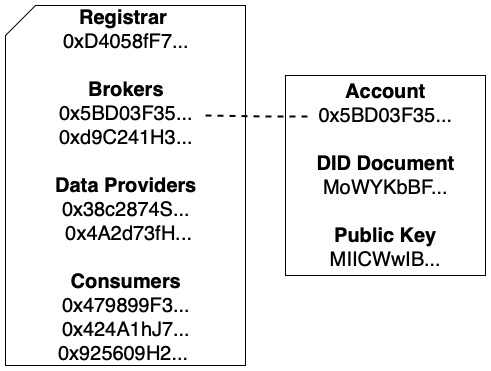
\includegraphics[width=0.4\textwidth]{registration_contract}
	\caption{Registration Contract.}
	\label{fig:registration_contract}
\end{figure}

\subsection{Launching and Searching Products}
To sell the sensing data, a data provider has to launch a new product on the data marketplace in advance. The data provider determines a trusted broker and asks the broker to create a new MAM channel and Product Contract (Figure \ref{fig:product_contract}).

\begin{figure}[h]
\centering
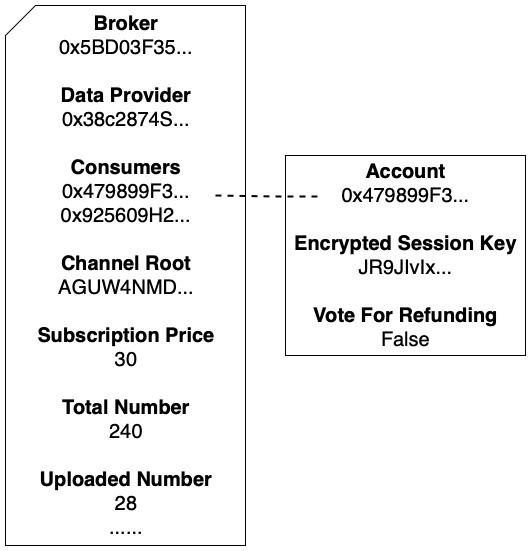
\includegraphics[width=0.4\textwidth]{product_contract}
\caption{Product Contract.}
\label{fig:product_contract}
\end{figure}

Brokers certify session keys as well. However, it is a risk revealing session keys to brokers since contents may be copied by brokers, which causes data providers' loss. Therefore, Blind signature is used to prevent the situation. Figure \ref{fig:key_certification} shows the certification process. When a data provider asks a broker to ceritfy new session key, the data provider uses the broker's public key, which is available in the Registration Contract after the broker's registration, as a blinding factor, and the session key is blinded. Then the data provider sends the blinded session key to the broker. The broker signs the message and returns the signature to data provider. The data provider removes the blinding factor and obtains the broker's signature of the session key. Only one session key can be signed in each product, so data providers can't fake a session key to deceive consumers.

\begin{figure}[h]
	\centering
	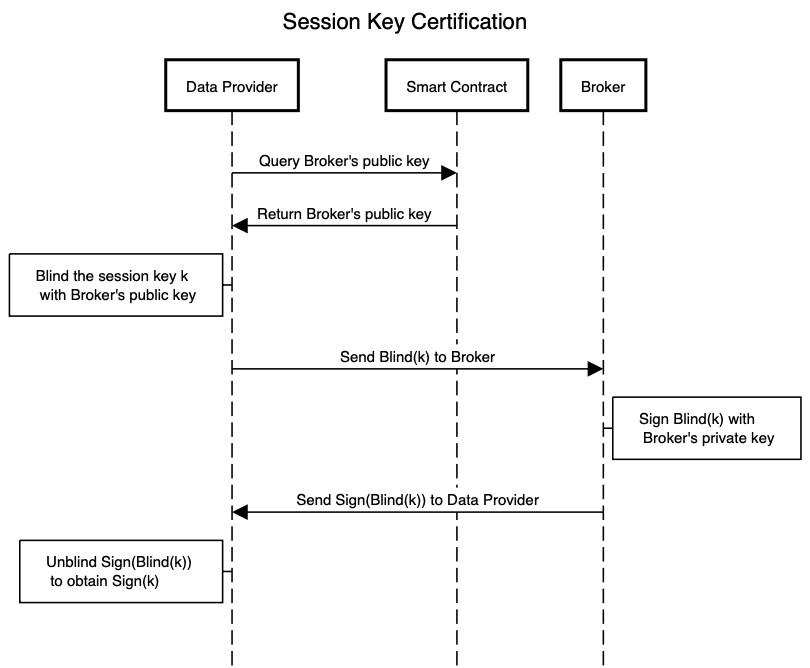
\includegraphics[width=0.5\textwidth]{key_certification}
	\caption{Session key certification process with blind signature.}
	\label{fig:key_certification}
\end{figure}

The contract address and product description will be stored in a file which is uploaded to IPFS. Consumers can search the desired product by keywords or tags. The consumer then evaluates the product and start trading with the data provider if the consumer is interested in subscribing the data.

\subsection{Trading}
Once a consumer who want to subscribe the sensor data pays a subscription fee to the Product Contract, it is added to the consumer list automatically by the smart contract. To decrypt the streaming data on the MAM channel, session key should be exchanged between data provider and consumers as shown in Figure \ref{fig:key_exchange}. The data provider requests the subscription list maintained by the Product Contract and obtains accounts of each consumer. After that, the data provider can also get public keys of each consumer from the Registration Contract with their accounts. For each consumer, the data provider encrypts the session key and broker's signature with the consumer's public key and sends the ciphertext to the Product Contract. Consumers listen to the smart contract event which is triggered when the ciphertext is updated, and decrypt the ciphertext to get the session key and signature. Consumers can obtain the broker's public key on the Registration Contract as well, so they can verify that the signature is valid and the session key is the only one that is certified by the broker. Afterward, encrypted sensing data is uploaded to the MAM channel, and consumers can download and decrypt them with the session key.

\begin{figure}[h]
	\centering
	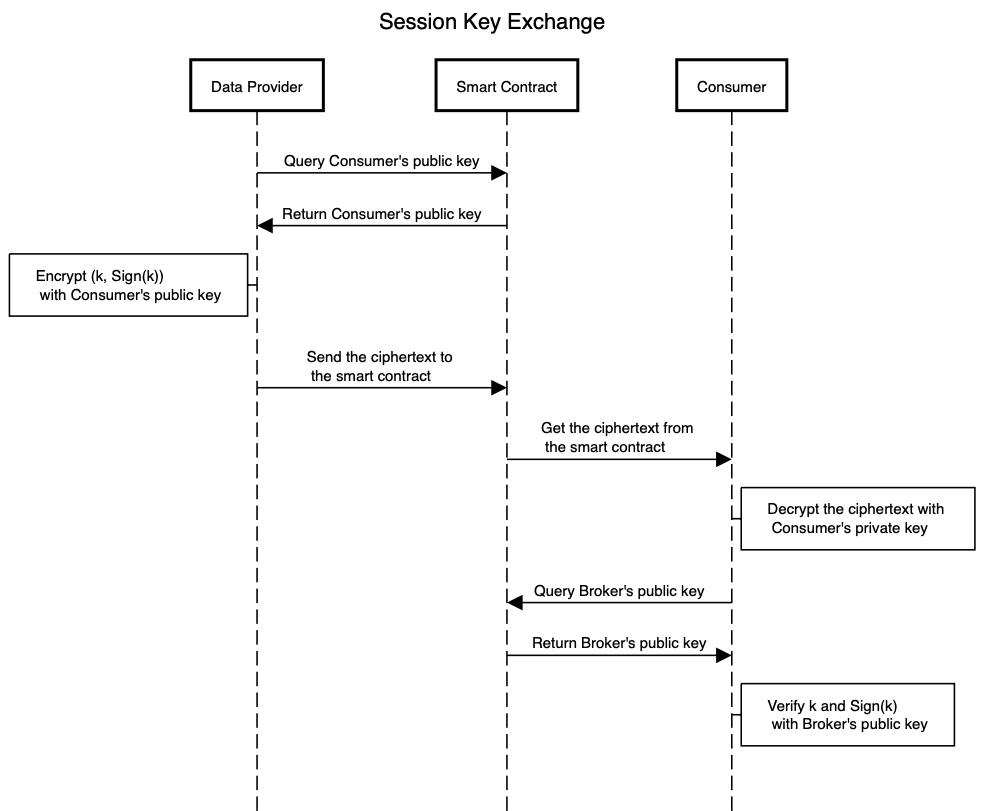
\includegraphics[width=0.5\textwidth]{key_exchange}
	\caption{Session key exchange process between the data provider and consumer.}
	\label{fig:key_exchange}
\end{figure}

\subsection{Refunding}
It is probable that the sensor is malfunctioning after the consumers pay the subscription fee. To protect consumers' right, the subscription fee are not transfered to the data provider until all data is generated and uploaded to the MAM channel. If the expected data is not available, consumers can ask for refunds. We assume that less than half of consumers in the Product Contract are irrational and malicious. Each consumer can vote for refunding at any time. If the ratio of consent votes of refunding is higher than the $threshold$ at $k$th piece of data, the subscription fee is proportionally transfered to the data provider, broker and every consumer. The subscription fee can be prorated as below:

\begin{equation}
F_{DataProvider}(k) = N price \frac{k-1}{M} (1-F_{b}) (1-F_{t})
\end{equation}

\begin{equation}
F_{Broker}(k) = N price \frac{k-1}{M} F_{b} (1-F_{t})
\end{equation}

\begin{equation}
F_{Consumer}(k) = price \frac{M-k+1}{M} (1-F_{t})
\end{equation}

where $price$  is the subscription price, $M$ is the number of expected data samples, $F_{b}$ is the brokerage fee(\%), $F_{t}$ is the transaction fee of the smart contract(\%), $N$ is the number of consumers in this contract.

To refund or withdraw subscription fee from the smart contract, data provider, broker, and consumer send a transaction to execute the smart contract and are responsible for transaction fee. We assume that only a half of the expected records are uploaded to the MAM channel. For the data provider and broker, they can withdraw a half of total subscription fee from the smart contract and $F_{b}$ \% belongs to the broker while the remaining belongs to the data provider. For consumers, they can get a half refund which should be deducted the transaction fee.



\subsection{Game Theory Evaluation}
\subsubsection{Repeated Game}
Repeated game consists of serveral repetitions of some stage games. In each stage game, the action player takes will effect the actions that players are going to take in the future stages. Repeated game can be illustrated with a decision tree and described their payoff with discounted sum of payoff. Discounted sum of payoff can capture the idea that what the players truly pursue is the sum of payoff in all stages and payoff in different stages may varify.

\subsubsection{Model Description}
We use a repeated game to express the scenario of our Data Marketplace. Figure.\ref{fig:decision_tree} shows the decision tree to depict the the repeated game we used. Each level in this decision tree represents each round of data transmission from data provider to data buyers, and the data buyers would pay subscription fee, $p_s$, each person. The sum of all the subscription fee pays to data provider is denoted as $P_s$.

Refund is a major issue in our research. However, we don't have to take refund as a factor in our repeated game, since in our decentralized data marketplace we use smart contract to store the subscription fee which will be paid to buy the future data. The subscription fee will be paid as data provider provides new data. In other words, data provide doesn't need to take any procedure to transer subscription fee from his/her own account to data buyers' account. For the same reason, data provider has no responsibility on the refunding processing fee charged by the smart contract as well.

\begin{figure} \centering 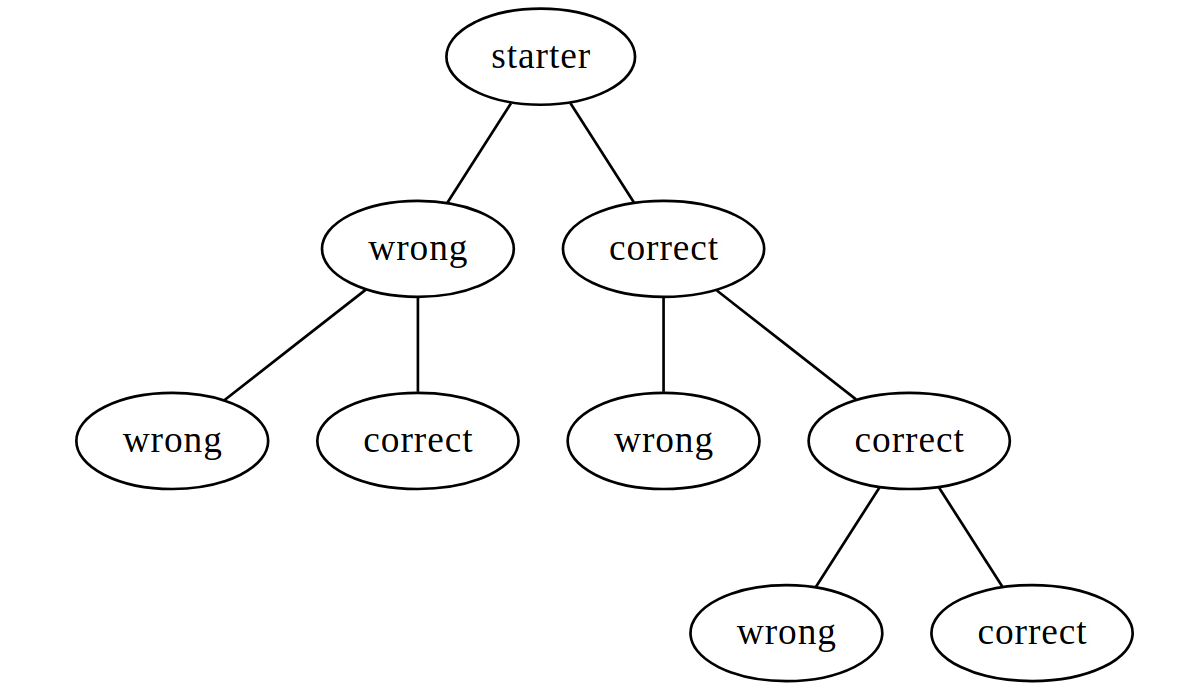
\includegraphics[width=3.3in]{img/decision_tree.png} \caption{Decision Tree}
    \label{fig:decision_tree} \end{figure}
For every $n$ round, the data provider would cost $C_{maintain}$ to maintain or enhance the sensors that data provider owns. We call this as a maintain period. Moreover, the value of data and the cost of maintenance will decrease as time pass, so we introduce a discounted factor $\beta$ to depict this phenomena.

We have these following assumptions:
\begin{itemize}
\item  There is no any other data providers provide the same product in Data Marketplace. Therefore, we can consider each provider's behavior independently. That means this decision tree represent the behavior of only one data provider.
\item  More than 51\% of data buyers are among complete information exchange state. In other words, once one of them launches voting for stopping buying data and refunding, they would succeed in refund voting.
\item  One of the data buyers who has complete information exchange with other 51\% buyers has the ability to examine the data quality. If unacceptably low accuracy data are delivered to data buyers, this examiner will spread this information out.
\end{itemize}

Based on the description above, the discounted sum of payoff for our repeated game is 
\begin{equation} \label{payoff}
\sum_{i=0}^{m}{\beta^{in}\cdot [(\sum_{j=0}^{n} \beta^j \cdot P_s) - C_{maintain}]}
\end{equation}

\begin{itemize}
\item $P_s$ is the sum of subscription price (fee) for all subscriber.
\item $C_{maintain}$ is the cost of sensor maintenance in $n$ round.
\item $\beta$ is discounted factor.
\item $n$ is how many round for one maintenance period.
\item $m$ is how many maintenance periods have been experienced in this repeated game.
\end{itemize}

Al-Fagih et al. presented\cite{DataPrice} $P_s$ is a sigmoid function of $P_r$, and based on rule of thumb $C_{maintain}$ is about a exponential function of $P_r$. We can substitute $P_s$ and $C_{maintain}$ with $P_r$ into Eq. (\ref{payoff}), then we can find out the Nash Equilibrium of repeated game easily.

\section{Conclusion}



  





% ---- Bibliography ----
\bibliographystyle{IEEEtran}
\bibliography{references}


\end{document}
